\documentclass[letterpaper,12pt,oneside]{article}
\usepackage[top=1in, left=1.25in, right=1.25in, bottom=1in]{geometry}
\usepackage[utf8]{inputenc}
\usepackage[spanish,es-nodecimaldot,es-tabla]{babel}
\usepackage{graphicx}
\usepackage{array}
\usepackage{natbib}
\bibliographystyle{plain}

\begin{document}
%\frontmatter
\begin{titlepage}
		\setlength{\parindent}{0pt} \setlength{\parskip}{0pt}
	
		\begin{center}
			\vfill 
			
			\begin{minipage}{\textwidth}
				
				\newcolumntype{V}{>{\centering\arraybackslash} m{.17\textwidth} }
				\newcolumntype{C}{>{\centering\arraybackslash} m{.56\textwidth} }
				
				\begin{center}
					
\includegraphics[width=4.5cm]{UNAM_LOGO2.png}	
				\end{center} 	
				\begin{center}
					\Huge\textbf{Universidad Nacional Autónoma de México}
				\end{center} 
				
			\end{minipage}
				
			\vfill
			
			\begin{minipage}{0.7\textwidth}
				\begin{center}
					\large Programa de Maestría en Ciencia e Ingeniería de la Computación
				\end{center}
			\end{minipage}
			% 
			\begin{center}
				%\medskip \rule{.9\textwidth}{2pt}
				\vfill
				\large TITULO DEL TRABAJO
				%{\Large \bfseries  \title   }
				
				%\medskip \rule{.9\textwidth}{2pt}
			\end{center}
			
			\begin{center}
				
				 PROTOCOLO DE INVESTIGACIÓN\\
			
				
				%PRESENTA:\\ \medskip
				\begin{center}
					P R E S E N T A \\
					\large NOMBRE DEL ALUMNO
				\end{center}
				
				\bigskip
				
				Tutor Principal\\
				Dr. NOMBRE APELLIDO, ADSCRIPCIÓN\\
				%Coadvisors
				Coasesor \\
                		Dr. NOMBRE APELLIDO, ADSCRIPCIÓN\\
			\end{center}
			
			\vfill
			
			\begin{center}
				{México, CDMX, MES 2023}\\
			\end{center}
			\cleardoublepage
		\end{center}
	\end{titlepage}
 
\clearpage
    
%\mainmatter

\section{Introducción} 

Describe de manera inicial la propuesta (¿Cuál es el problema?, ¿Hay alguna solución existente? ¿Cuáles?, ¿Cuál funciona mejor?, ¿Cuáles son las limitaciones de las soluciones existentes?, ¿Cómo espera contribuir?, párrafo de 2000 a 5000 caracteres). Este párrafo debe incluir la justificación y el planteamiento del problema y las contribuciones \cite{phil99}. Se deben incluir referencias \cite{smit54, jame76}.

\section{Estado del arte}
Se refiere al conocimiento previo de teorías, avances científicos y/o tecnológicos que soportan la Investigación a desarrollar (Descripción del problema, Necesidad, Motivación para atenderlo, Estado actual del campo: ¿Hay alguna solución existente?¿Cuáles?, ¿Cuál funciona mejor?, Se enunciarán los fundamentos teóricos y se describirán las variables, párrafo de 2000 a 5000 caracteres \cite{gree00}). Aquí se espera encontrar varias citas \cite{colu92}. 

\section{Objetivo general}
Describe el alcance general de la investigación a desarrollar (El enunciado que expresa el objetivo, siempre escribir como primera palabra un verbo en infinitivo, es decir aquellos con terminaciones ar, er, ir. Responde a las preguntas: ¿Qué se va hacer?, ¿Mediante qué o cómo se va hacer?, ¿Para qué se va hacer?)

\section{Objetivos particulares}
Precisan las acciones que se llevarán a cabo para lograr el objetivo general (Los objetivos específicos son los resultados y beneficios cuantificables esperados cuando se lleva a cabo una estrategia. Responden a la pregunta: ¿Qué va a lograr cada estrategia?. Deben cumplir los siguientes requisitos: Medibles, que permitan su seguimiento y evaluación. Apropiados a los problemas, Objetivos generales y Estrategias. Temporales, con un periodo de tiempo específico para alcanzarlos. Realistas, es decir, alcanzables, con sentido, desafiantes.)

\section{Metodología propuesta}
Deberá describir el o los procedimientos científico-metodológicos a seguir para cumplir con los objetivos y metas del proyecto, indicando las técnicas, el diseño experimental y las pruebas estadísticas a utilizar (Se explicarán los procedimientos científicos, tecnológicos, de laboratorio, normas aplicables y análisis estadísticos que se seguirán para cumplir los objetivos y metas del proyecto. Métodos: Debe mostrar los detalles para que se pueda reproducir el trabajo. Se pueden presentar por importancia o en forma cronológica. Diseño experimental. Reportar lo que se va a utilizar. Reportar como se hicieron los experimentos; métodos y técnicas. Análisis  de datos, métodos de cuantificación, pruebas estadísticas.)

\section{Programa de actividades} 
Se definen actividades a desarrollar, los productos entregables, el periodo de realización, etc. Se enunciarán las actividades por desarrollar durante cada una de las etapas del proyecto, así como los tiempos en que se realizarán. Se recomienda usar una tabla tipo Gantt Chart.

\begin{figure}[h]
    \centering
    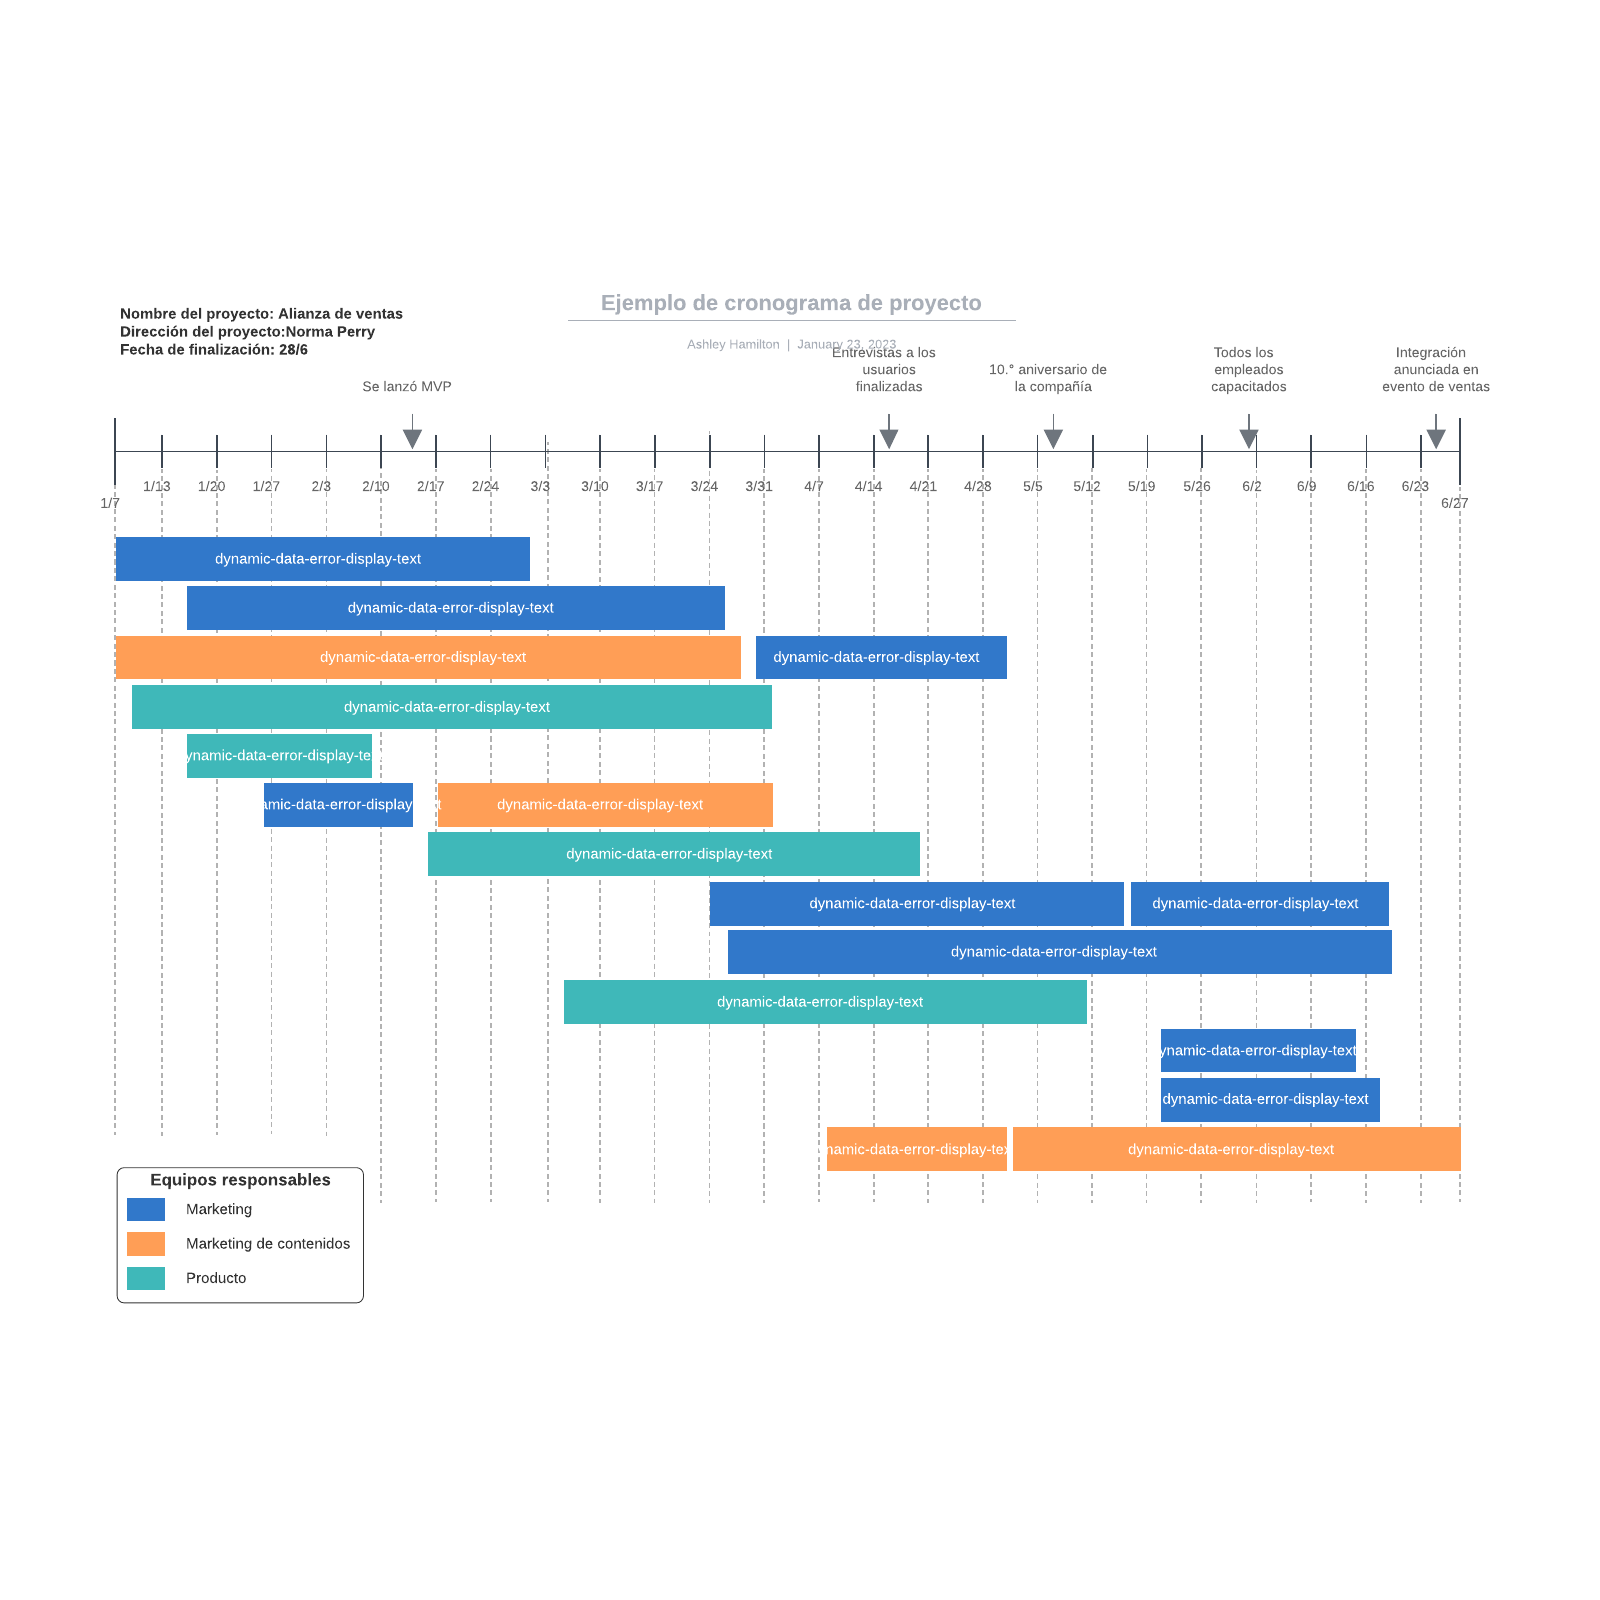
\includegraphics[scale=0.5]{cronograma.png} %Poner el nombre de tu imagen
    \caption{Programa de actividades}
    \label{fig:cron}
\end{figure}

\bibliography{mybibliography.bib} %Se asume que se tiene el archivo mybibliography.bib
\end{document}
